\documentclass{article}

% Formatting
\usepackage[utf8]{inputenc}
\usepackage[margin=1in]{geometry}
\usepackage[titletoc,title]{appendix}
\usepackage[spanish]{babel}
\usepackage{amsmath,amsfonts,amssymb,mathtools}
\usepackage{graphicx,float}
\usepackage[ruled,vlined]{algorithm2e}
\usepackage{algorithmic}
\usepackage{minted}
\usemintedstyle{borland}
\usepackage{biblatex}
\usepackage{subcaption}

% Title content
\title{Práctica 2 Autómata Celular}
\author{Denisse leyva}
\date{Febrero 24, 2021}

\begin{document}

\maketitle

% Introduction
\section{Introducción}
En esta segunda practica trabajaremos con autómatas celulares en dos dimensiones, particularmente el famoso juego de la vida. Eel estado del autómata se representa con una matriz booleana (es decir, contiene ceros y unos). Cada celda es o viva (uno) o muerta (cero). En cada paso, la supervivencia de cada celda (verde) se determina a partir de los valores de sus ocho vecinos (amarillos):\\

\begin{figure}[H]
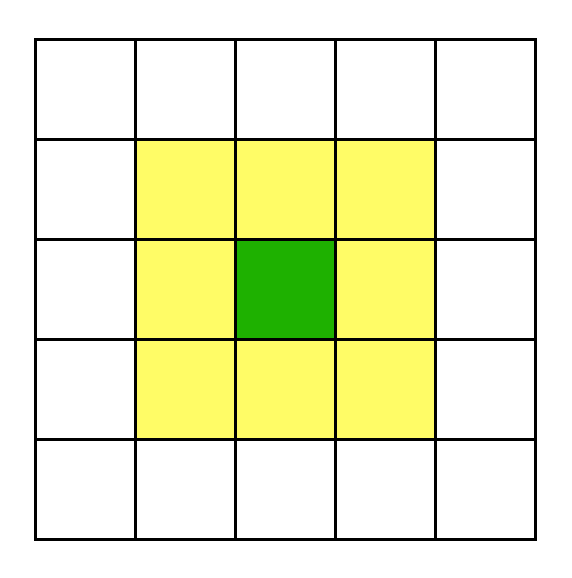
\includegraphics[width=40mm]{p2v.png}
\end{figure}

En los extremos de la matriz, las celdas simplemente tienen menos vecinos. (Otra alternativa seria considerar el espacio como un torus -pareciendo una dona- donde el extremo de abajo se reúne con el extremo de arriba igual como los lados izquierdo y derecho uno con otro.\\
La regla de supervivencia es sencilla: una celda está viva si exactamente 3 vecinos suyos están vivos.[1]


\section{Objetivo}
Se debe diseñar y ejecutar un experimento para determinar el efecto de la regla de supervivencia (por lo menos 5 reglas) en la vida de la colonia en una malla de 12 por 12 celdas hasta que se mueran todas o que se hayan cumplido las 30 iteraciones, teniendo cada celda o viva o muerta con la misma probabilidad al inicio. Graficar y tabular los hallazgos.[1]

\section{Código}
Se debe diseñar y ejecutar un experimento para determinar el efecto de la regla de supervivencia (por lo menos 5 reglas) en la vida de la colonia en una malla de 12 por 12 celdas hasta que se mueran todas o que se hayan cumplido las 30 iteraciones, teniendo cada celda o viva o muerta con la misma probabilidad al inicio. Graficar y tabular los hallazgos[1]\\
Con el siguiente código se realizan 5 reglas de supervivencia con el fin de graficar su comportamiento de vida durante 30 iteraciones.\\
La primera regla que se ejecuta es la regla general u obligatoria de 3 vecinos para vivir. La segunda regla parte de la esencia de la primera regla que vive con 3 vecinos, pero tiene un 50 por ciento de probabilidad de vivir con 4 y 2 vecinos, con más o menos vecinos muere.\\
La tercera regla sigue siendo una extensión de la primera y la segunda ya que en base al comportamiento de la segunda regla de si en la primera iteración logro vivir con 2 o 4 vecinos tendrá la oportunidad de no morir con 1 o 5 hasta 8 vecinos, esto pretendiendo suponer que tiene la posibilidad de ser inmortal.
\\

La cuarta regla ya se independiza de las primeras 3 dando diferentes probabilidades de vida según la cantidad de vecinos que tiene.\\


 \begin{tabular}{||c c ||} 
 \hline
 Vecinos & Porcentaje de Vida  \\ [0.5ex] 
 \hline\hline
 0 & 01\% \\
 \hline
 1 & 20\% \\ 
 \hline
 2 & 30\%  \\
 \hline
 3 & 50\% \\
 \hline
 4 & 35\% \\
 \hline
 5 & 60\% \\ [1ex] 
 \hline
 6 & 05\% \\
 \hline
 7 & 85\% \\
 \hline
 8 & 02\% \\
 \hline
\end{tabular}
\\

La quinta y última regla nos dice que si tienes un número par de vecinos se tiene el 50 por ciento de probabilidad de vivir y con número impar solo se tiene el 1 por ciento de probabilidad de vida.

Para este código se usó la alternativa de considerar el espacio como un torus (pareciendo una dona). Y se usó el código base de la Dra. Elisa Schaeffer que se obtuvo de su repertorio de GitHub[2]\\

**Código creado en Python**

\begin{verbatim}
import numpy as np 
from random import random
import matplotlib.cm as cm
import matplotlib.pyplot as plt


dim = 12
num = dim**2
p = 0.5
valores = [1*(random() < p) for i in range(num)]
print(valores)
actual = np.reshape(valores,(dim,dim))
print("El actual es: ", actual)
valor_a = []

def mapeo(pos):
    fila = pos // dim
    columna = pos % dim
    return actual[fila, columna]

assert all([mapeo(x) == valores[x] for x in range(num)])


def paso(pos, reglas):
    fila = pos // dim
    columna = pos % dim
    actual_o = actual
    if fila == 0:
        actualn = actual_o[[dim-1],:]
        actualm = actual_o[[i for i in range(dim-1)],:]
        actual_o = np.append(actualn,actualm, axis=0)
        fila += 1

    elif fila == dim-1:
        actualn= actual_o[[0],:]
        actualm= actual_o[[i for i in range(1,dim)],:]
        actual_o = np.append(actualm,actualn, axis=0)
        fila -= 1

    if columna == 0:
        actualn= actual_o[:,[dim-1]]
        actualm= actual_o[:,[i for i in range(dim-1)]]
        actual_o = np.append(actualn,actualm, axis=1)
        columna += 1

    elif columna == dim-1:
        actualn= actual_o[:,[0]]
        actualm= actual_o[:,[i for i in range(1,dim)]]
        actual_o = np.append(actualm,actualn, axis=1)
        columna -= 1

        
    vecindad = actual_o[max(0, fila -1):min(dim, fila + 2),
              max(0, columna -1):min(dim, columna +2)]
    actual_f=actual_o
    actual_o=actual
    vecinos = (np.sum(vecindad) - actual_f[fila, columna])

    if reglas == 1:
        return 1 * (vecinos == 3)
    
    elif reglas == 2:
        if vecinos == 3:
            regla = True
            
        elif vecinos == 2:
            regla = 1 * (random() < 0.5)
        elif vecinos == 4:
            regla = 1 * (random() < 0.5)
        else:
            regla = False
           
        return 1 * (regla)
    
    elif reglas == 3:
        valor_a.append(valores[pos])
        
        if vecinos == 3:
            regla = True
            
        elif vecinos == 2:
            
            if valor_a[pos] == 1:
                regla = True
            else:
                regla = 1 * (random() < 0.5)

        elif vecinos == 4:
 
            if valor_a[pos] == 1:
                regla = True

            else:
                regla = 1 * (random() < 0.5)

        else:
            regla = False

        return 1 * (regla)
        
    elif reglas == 4:
        if vecinos == 1:
            regla = 1 * (random() < 0.2)
            
        elif vecinos == 2:
            regla = 1 * (random() < 0.3)
        
        elif vecinos == 3:
            regla = 1 * (random() < 0.5)
        
        elif vecinos == 4:
            regla = 1 * (random() < 0.35)
        
        elif vecinos == 5:
            regla = 1 * (random() < 0.6)
        
        elif vecinos == 6:
            regla = 1 * (random() < 0.05)
        
        elif vecinos == 7:
            regla = 1 * (random() < 0.85)
        
        elif vecinos == 8:
            regla = 1 * (random() < 0.02)
        
        else:
            regla = 1 * (random() < 0.01)
        
        return 1 * (regla)
    
    
    elif reglas == 5:
        if vecinos % 2 == 0:
            regla = 1 * (random() < 0.5) 
        else:
            regla = 1 * (random() < 0.01)
        
        return 1 * regla
    else:
        print("El numero de regla no existe")
        return 1 * False
        
if __name__ == "__main__":
    vi_t = []
    for reglas in range(1,6):
        fig = plt.figure()
        plt.imshow(actual, interpolation='nearest', cmap=cm.Greys)
        fig.suptitle('Estado inicial')
        
        va, vi =  [], []
        plt.savefig('p2_r{:d}_t0_p.png'.format(reglas))
        plt.close()
        plt.show()
        actual_i = actual
        # print(actual_i)
        valores_i = valores
        vivos = sum(valores)
        vi.append(vivos)
        for iteracion in range(30):
            
            valores = [paso(x,reglas) for x in range(num)]
            va.append(valores)
            
            vivos = sum(valores)
            vi.append(vivos)
            # print(vi)
            if vivos == 0:
                print('# Ya no queda nadie vivo.')
                break;
            actual = np.reshape(valores, (dim, dim))
            fig = plt.figure()
            plt.imshow(actual, interpolation='nearest', cmap=cm.Greys)
            fig.suptitle('Paso {:d}'.format(iteracion + 1))
            plt.savefig('p2_r{1:d}_t{0:d}_p.png'.format((iteracion + 1),reglas))
            plt.close()
            plt.show()
        actual = actual_i
        valores = valores_i
        vi_t.append(vi)
    print(vi_t)
    fig, (ax1, ax2, ax3, ax4, ax5) = plt.subplots(5, sharex= True, sharey = True)
    fig.suptitle('Graficas de vida durante las iteraciones, de la regla 1 a la 5')
    ax1.plot(vi_t[0])
    ax2.plot(vi_t[1])
    ax3.plot(vi_t[2])
    ax4.plot(vi_t[3])
    ax5.plot(vi_t[4])
    plt.savefig('Grafica de vida')
# print(va)

\end{verbatim}
\newpage
En la siguiente imagen se puede apreciar el comportamiento de la gráfica con las 5 reglas en sus 30 iteraciones.

\begin{figure}[H]
\centering
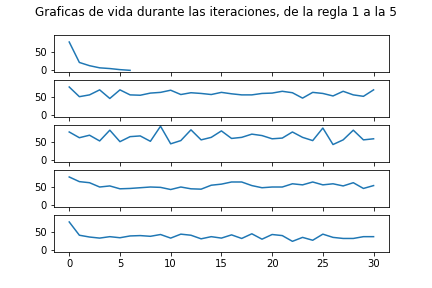
\includegraphics[width=120mm]{Grafica de vida.png}
\caption{\label{fig1}Gráfica de las 5 reglas de supervivencia.}
\end{figure}

A continuación, se muestran el estado inicial y final del comportamiento de la matriz para cada regla.

\begin{figure}[h!]
\centering
\begin{subfigure}[b]{0.45\linewidth}
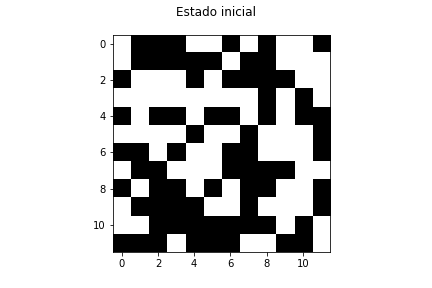
\includegraphics[width=\linewidth]{p2_r1_t00_p.png}
\caption{Estado Inicial}
\end{subfigure}
\begin{subfigure}[b]{0.45\linewidth}
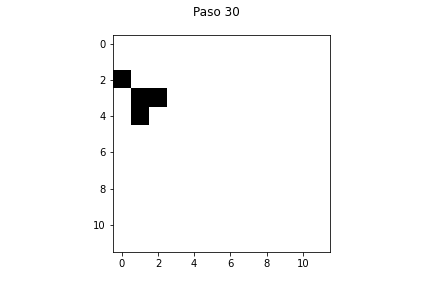
\includegraphics[width=\linewidth]{p2_r1_t30_p.png}
\caption{Estado Final}
\end{subfigure}
\caption{Imagen del estado inicial y final de la Regla 1 de supervivencia}
\label{fig:westminster}
\end{figure}


\begin{figure}[H]
\centering
\begin{subfigure}[b]{0.45\linewidth}
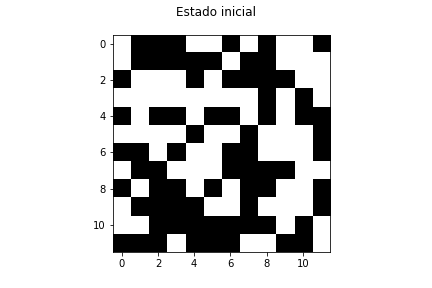
\includegraphics[width=\linewidth]{p2_r2_t00_p.png}
\caption{Estado Inicial}
\end{subfigure}
\begin{subfigure}[b]{0.45\linewidth}
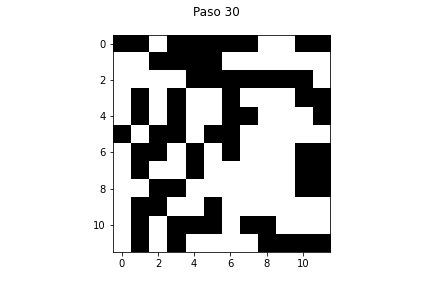
\includegraphics[width=\linewidth]{p2_r2_t30_p.png}
\caption{Estado Final}
\end{subfigure}
\caption{Imagen del estado inicial y final de la Regla 2 de supervivencia}
\label{fig:westminster}
\end{figure}

\begin{figure}[H]
\centering
\begin{subfigure}[b]{0.45\linewidth}
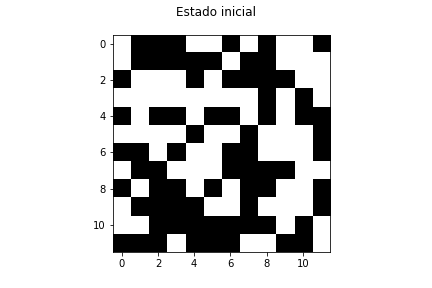
\includegraphics[width=\linewidth]{p2_r3_t00_p.png}
\caption{Estado Inicial}
\end{subfigure}
\begin{subfigure}[b]{0.45\linewidth}
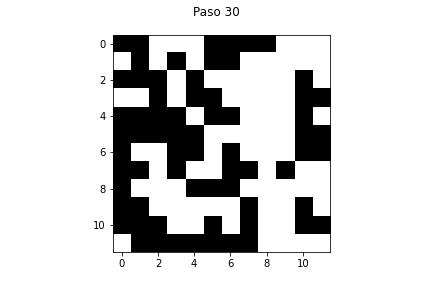
\includegraphics[width=\linewidth]{p2_r3_t30_p.png}
\caption{Estado Final}
\end{subfigure}
\caption{Imagen del estado inicial y final de la Regla 3 de supervivencia}
\label{fig:westminster}
\end{figure}

\begin{figure}[H]
\centering
\begin{subfigure}[b]{0.45\linewidth}
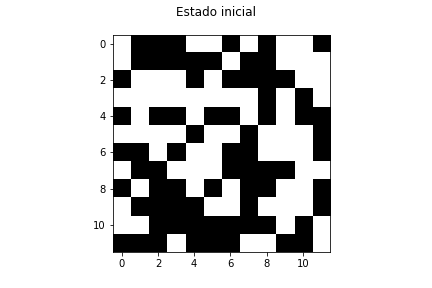
\includegraphics[width=\linewidth]{p2_r4_t00_p.png}
\caption{Estado Inicial}
\end{subfigure}
\begin{subfigure}[b]{0.45\linewidth}
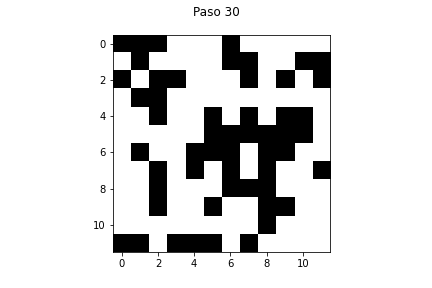
\includegraphics[width=\linewidth]{p2_r4_t30_p.png}
\caption{Estado Final}
\end{subfigure}
\caption{Imagen del estado inicial y final de la Regla 4 de supervivencia}
\label{fig:westminster}
\end{figure}

\begin{figure}[H]
\centering
\begin{subfigure}[b]{0.45\linewidth}
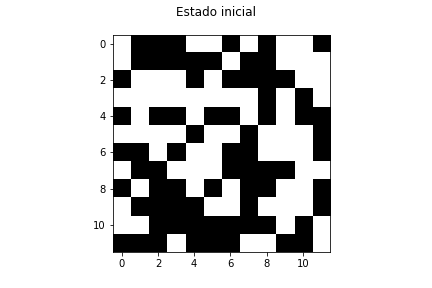
\includegraphics[width=\linewidth]{p2_r5_t00_p.png}
\caption{Estado Inicial}
\end{subfigure}
\begin{subfigure}[b]{0.45\linewidth}
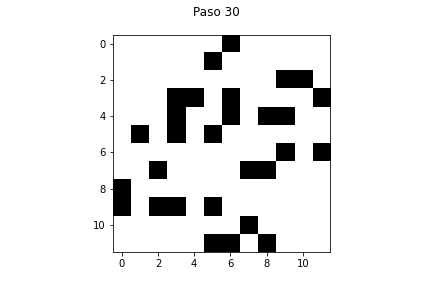
\includegraphics[width=\linewidth]{p2_r5_t30_p.png}
\caption{Estado Final}
\end{subfigure}
\caption{Imagen del estado inicial y final de la Regla 5 de supervivencia}
\label{fig:westminster}
\end{figure}


\section{Reto 1}

\begin{thebibliography}{99} %% use BibTeX or add references manually

\bibitem{ESchaeffer} Elisa Schaeffer. Práctica 2 Febrero 2021
\url{https://elisa.dyndns-web.com/teaching/comp/par/p2.html}.

\bibitem{ESchaeffer} Elisa Schaeffer. ejemplo gameOfLife.py Febrero 2021
\url{https://github.com/satuelisa/Simulation/blob/master/CellularAutomata/gameOfLife.py}.


\end{thebibliography}

\end{document}
